\section{Benutzer Client}

	\subsection{UML2-Komponentendiagramm}

		\begin{figure}[H]
    		\centering
    		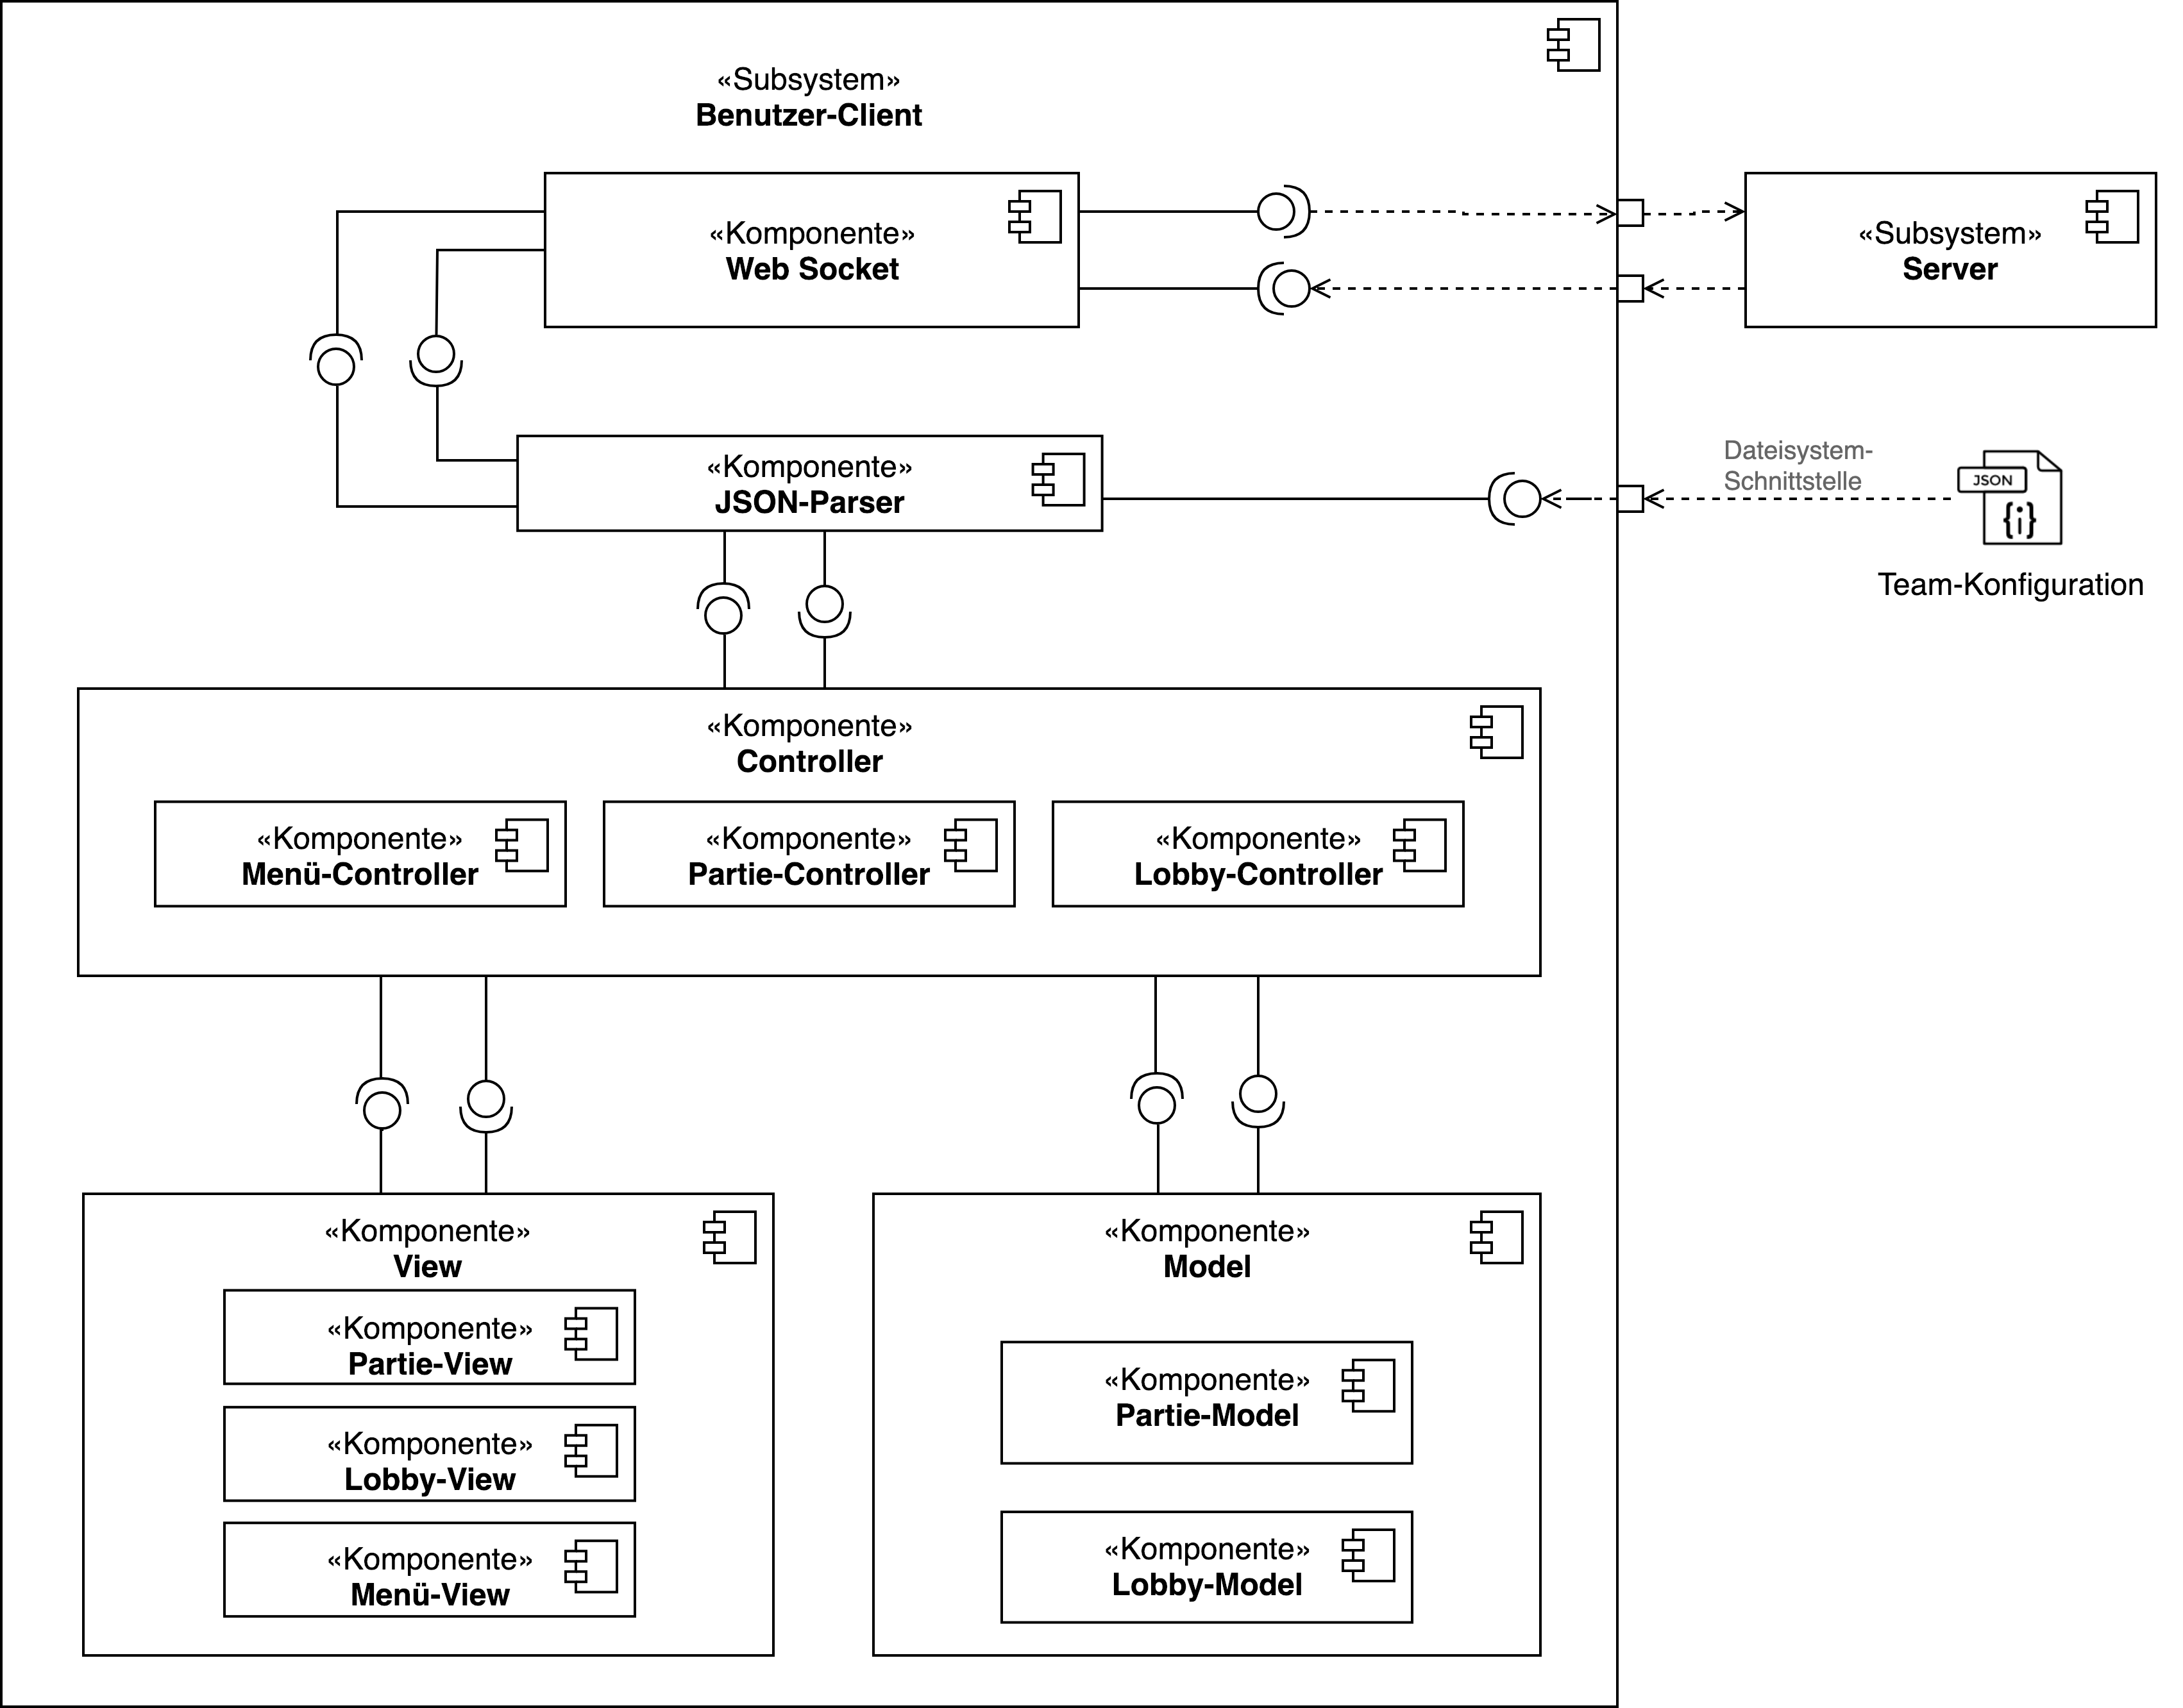
\includegraphics[scale=0.5]{images/komponentendiagramm_benutzer-client.png}
		\end{figure}

	\subsection{Beschreibungen}

		\begin{description}
			
			\item[Benutzer-Client]
			Beim Benutzer-Client handelt es sich um eine Anwendung mit grafischer Benutzeroberfläche mit der \textit{Flappy Wizard}-Partien beigetreten werden kann und diese auf verschiedene Weisen verfolgt werden können. In einer Lobby können Partien auf einem Server erstellt werden oder es kann einer bestehenden Partie auf einem Server beigetreten werden. Die Spiellogik einer Partie läuft jedoch stets auf dem Server. Eine Partie lässt sich sowohl passiv als Beobachter verfolgen als auch aktiv als Spieler gestalten. In diesem Fall nimmt der Benutzer-Client Spieleraktionen entgegen und sendet sie an den Server.
			\item[Controller]
			Der Controller ist die Schaltstelle aller Aktionen im Benutzer-Client.			
			
			\begin{description}
				\item[Menü-Controller]
				Der Menü-Controller beinhaltet die Logik, mit der im Menü zwischen verschiedenen Ansichten hin und her gewechselt werden kann.
			
				\item[Spiel-Controller]
				Der Spiel-Controller hat zwei Aufgaben. Einerseits behandelt er alle Ereignisse und Nutzereingaben, die über die Spiel-View bereitgestellt werden und leitet sie an das Modell bzw. den Server weiter. Andererseits nimmt er Spieldaten vom Server bzw. dem JSON-Parser entgegen und aktualisiert damit die Partie-View und das Partie-Model des Benutzer-Clients.
			
			
				\item[Lobby-Controller]
				Mit dem Lobby-Controller werden die Interaktionen in der Lobby zwischen Server, Benutzer-Client-Anwendung und Nutzereingaben behandelt. Insbesondere bietet er eine Schnittstelle zum Dateisystem, wodurch eine Team-Konfiguration ausgewählt werden kann.
			\end{description}
			
			\item[View]
			Die View enthält alle Klassen, die die grafische Benutzeroberfläche des Benutzer-Clients bilden. Sie unterteilt sich in die drei Komponenten Menü-View, Lobby-View und Partie-View.
			\begin{description}
				\item[Partie-View]
				Die Partie-View enthält alle Klassen, die die grafische Darstellung einer Partie sowohl im Beobachter- als auch im Spieler-Modus ausmachen. Nutzereingaben und Ereignisse werden an den entsprechenden Controller weitergeleitet.
			
			
				\item[Lobby-View]
				Die Lobby-View enthält alle Klassen, die zur grafischen Darstellung der Partie-Lobby notwendig sind. Nutzereingaben werden an den entsprechenden Controller weitergeleitet.
			
			
				\item[Menü-View]
				Die Menü-View enthält alle Klassen, die zur grafischen Darstellung des Menüs notwendig sind. Nutzereingaben werden an den entsprechenden Controller weitergeleitet.

			\end{description}
			
			
			
			\item[Model]
			Das Model ist eine Gruppe von Klassen, die wichtige Zustände des Benutzer-Clients repräsentieren.
			
			\begin{description}
				\item[Lobby-Model]
				Das Lobyy-Model fasst die Klassen zusammen, die die Zustände der Lobby repräsentieren. Dazu gehören zum Beispiel vorhandene Partien und beigetretene Spieler bzw. Beobachter.
			
				\item[Partie-Model]
				Das Partie-Model enthält alle Klassen, die eine Partie vollständig repräsentieren. Es wird regelmäßig mit dem Server und den Nutzereingaben synchronisiert.
			\end{description}
			
			\item[Web Sockets]
			Der Web Socket bildet die Komponente, die sich um die Datenübertragung mit dem Server kümmert. Daten über den Spielzustand werden vom Server empfangen und Spieleraktionen werden an den Server gesendet.
			
			\item[JSON-Parser]
			Der JSON-Parser wandelt die JSON-Daten in interne Objekte der Software um und umgekehrt. Da auch in den Client-Anwendungen eine ähnliche Komponente von Nöten ist, bietet es sich an diese Funktionalitäten in einer eigenen Komponente auszulagern.  

		\end{description}
		
	\subsection{Zuordnung der Funktionalen Anforderungen}
	
	Die funktionalen Anforderungen gemäß dem Pflichtenheft werden den Komponenten folgendermaßen zugeteilt:

	\begin{tabular}{|l|l|}
		\hline
		\textbf{Komponente} & \textbf{Abgedeckte funktionale Anforderungen}\\ \hline
		Menü-Controller & FA56 \\ 
		& FA60 \\
		& FA65 \\
		& FA67 \\ \hline
		
		Lobby-Controller & FA61 \\
		& FA56 \\
		& FA63 \\
		& FA67 \\ \hline
		
		Partie-Controller & FA56 \\
		&  FA67-69 \\
		
		Menü-View & FA56 \\ 
		& FA60 \\
		& FA65 \\ \hline
		
		Lobby-View & FA61 \\ 
		& FA63 \\ \hline
		
		Partie-View & FA62 \\ 
		& FA64 \\ 
		& FA66 \\ \hline
		
		Partie-Model & FA01-52 \\ 
		& FA60 \\
		& FA65 \\ \hline
		
		Lobby-Model & FA61 \\ 
		& FA63 \\
		& FA65 \\ \hline
		
		Web Socket & FA55 \\ \hline
		
		JSON-Konverter & FA53 \\
		& FA57\\ \hline
	
\end{tabular}